In this chapter, we outline the implementation of our NMOps architecture, as described in \ref{fig:nmops-architecture}, incorporating best practices from MLOps frameworks, as summarized in \ref{MLOPS}, and the algorithm presented in section \ref{alg:algorithm}.

Some of the process, usage, and requirements of the NMOps are given below:
\begin{enumerate}
    \item \textbf{Data pipeline:}\begin{itemize}
        \item \textbf{Ingestion:} Connect to Azure Data Lake to pull battery telemetry (cycles, voltage, current, temperature) in batch mode.
        \item \textbf{Preprocessing:} Automate scaling and window size computation using a workflow orchestrator. Store pre-computed mean for efficiency. Validate data quality (no missing values, numerical consistency).
        \item \textbf{Scheduling:} Run daily or event-triggered preprocessing jobs to handle new data.
        \item \textbf{Tools:} Kuberflow, Pandas/Spark for transformations.
    \end{itemize}
    \item \textbf{Model Training Pipeline:} \begin{itemize}
        \item \textbf{Training:} Encapsulate MHE, stacking, and EKF optimization in a training pipeline. Log parameters ($k_1$, $k_2$, regression weights, Q, R, trend\_rate) and metrics (MSE, RMSE) using MLflow. Support parallel training with Dask or Spark.
        \item \textbf{Hyperparamete Tuning:} Automate Optuna runs for MHE and EKF, storing best paramters in a MLflow model registry.
        \item \textbf{Frequency:} Train weekly or when data drift is detected. 
        \item \textbf{Tools:} MLflow for logging, SageMaker for cloud training, Kuberflow for orchestration.
    \end{itemize}
    \item \textbf{Model Deployment}: \begin{itemize}
        \item \textbf{Serving:} Deploy a REST API or serverless function to correct SOH in real-time.
        \item \textbf{Batch Inference:} Support batch processing for historical data using scheduled jobs.
        \item \textbf{Model Registry:} Store trained models (linear regression weights, $k$ values, EKF parameters) with versioning.
        \item \textbf{Scaling:} Auto-scaling to handle variable loads.
        \item \textbf{Tools:} FastAPI for API, Docker for containerization, Kubernetes for orchestration.
    \end{itemize}
    \item \textbf{Monitoring and Maintenance:} \begin{itemize}
        \item \textbf{Performance Monitoring:} Track RMSE\_ground\_truth and \\ RMSE\_final\_cyclic daily using a dashboard. Alert if RMSE>5\% (indicating correction degradation).
        \item \textbf{Data Drift:} Monitor Final\_cyclic\_againg\_scaled distribution for shifts (e.g., mean change > 10\%).
        \item \textbf{Model Drift:} Compare predictions against new ground truth data to detect performance drops.
        \item \textbf{Logging:} Log API requests, prediction errors, and retraining events to a centralized system.
        \item \textbf{Tools:} Grafana for dashboards, Prometheus for alerts.
    \end{itemize}
    \item \textbf{CI/CD and Retraining:}\begin{itemize}
        \item \textbf{Continuous Integration:} Automate testing of code updates using GitHub Actions.
        \item \textbf{Continuous Delivery:} Deploy updated models to production endpoints when retrained with rollback support via model registry.
        \item \textbf{Retraining Triggers:} Retrain on new data weekly, when RMSE>5\%, or when drift is detected.
        \item \textbf{Tools:} GitHub Actions for CI, Jenkins for CD, MLflow for model versioning.
    \end{itemize}
    \item \textbf{Infrastructure:} \begin{itemize}
        \item \textbf{Cloud:} Deploy on Azure with managed services.
        \item \textbf{Containerization:} Package algorithm in Docker containers for consistent deployment.
        \item \textbf{Orchestration:} Use Kubernetes for scaling and managing API services.
    \end{itemize}
    \item \textbf{Operational Requirements:}\begin{itemize}
        \item \textbf{Deployment:} Support batch processing for historical data and real-time API for live SOH correction. Ensure 99.9\% uptime for production APIs, with auto-scaling in cloud environments.
        \item \textbf{Monitoring:} Monitor RMSE\_ground\_truth daily, alerting if >5\%. Track data drift in the Final cyclic aging scaled. Log model performance and retraining events in the dashboard.
        \item \textbf{Maintenance:} Schedule weekly retraining or when drift is detected. Update the correction logic based on feedback. Maintain documentation and version control.
    \end{itemize}
    \item \textbf{Constraints and Assumptions:} \begin{itemize}
        \item \textbf{Constraints:} \begin{itemize}
            \item Limited to numerical cycle data with no missing values.
            \item Sequential processing limits scalability; large-scale use requires parallelization.
            \item Optuna optimization is CPU-bound, slowing down large datasets.
        \end{itemize}
        \item \textbf{Assumptions:} \begin{itemize}
            \item Final cycling aging is a semi-empirical SOH estimate, reasonably accurate.
            \item Ground truth SOH is available for training and validation.
            \item Battery data is clean and representative of EV/storage use cases.
            \item Cloud resources are available for scaling.
        \end{itemize}
    \end{itemize}
\end{enumerate}

The battery SOH estimation project requires robust requirements to deliver accurate, scalable, and maintainable predictions. Correcting semi-empirical SOH estimates using MHE, stacking, and EKF supports critical applications, such as electric vehicle (EV) fleet management. Integration into an MLOps architecture—via automated data pipelines, training, deployment, monitoring, and continuous integration/continuous deployment (CI/CD)—ensures continuous improvement and reliability in production. With parallelization, distributed computing, and MLOps tools, it scales to large datasets and fits seamlessly into modern ML workflows.

\subsection{Dataset}

This study utilizes the NASA Lithium-Ion Battery Dataset, made publicly available by the Prognostics Center of Excellence (PCoE) at NASA Ames Research Center. The dataset has become a benchmark for researching battery health diagnostics, performance forecasting, and remaining useful life (RUL) prediction. It is widely adopted in both academic and industrial settings.

The dataset contains time-series data collected from commercial lithium-ion cells operated under controlled test conditions until they reached their end-of-life, which is defined as the point where battery capacity falls below 70\% of the rated nominal value. Each battery was subjected to repeated charge–discharge cycles, during which parameters such as voltage, current, temperature, and capacity were continuously recorded.

The batteries were tested under various cycling protocols to simulate real-world degradation behavior, including different charge/discharge currents and thermal environments. This results in diverse degradation trajectories across the dataset, which helps in training and validating robust predictive models.

The dataset is particularly valuable due to its incorporation of practical challenges such as sensor noise, non-linear aging behavior, and inter-cycle variability. These characteristics make it suitable not only for capacity forecasting but also for tasks like fault detection, anomaly identification, and model generalization. As such, the NASA dataset provides a realistic and comprehensive testbed for developing and evaluating algorithms for battery prognostics and health management.


\subsubsection{Dataset Structure}
Figure \ref{fig:data-structure} illustrates the structure of the NASA dataset used. The data is grouped by battery. Each battery (e.g., B005) has its dataset. For each battery, the entire life of the battery is divided into individual charge-discharge cycles. Each cycle contains the cycle number, charge data, discharge data, capacity measurement, and time stamps. The recorded data included Voltage (V), Current (A), Temperature (\degree C), and Capacity (Ah). Batteries were considered to have failed when their capacity dropped to 70\% of their nominal capacity (2.0 Ah).

\subsubsection{Testing Conditions}
The batteries were cycled under different operating conditions, including varying charge/discharge rates (C-rates), temperature variations, and different state-of-charge windows (e.g., charging between 4.2 V and 2.5 V)

\begin{figure}
    \centering
    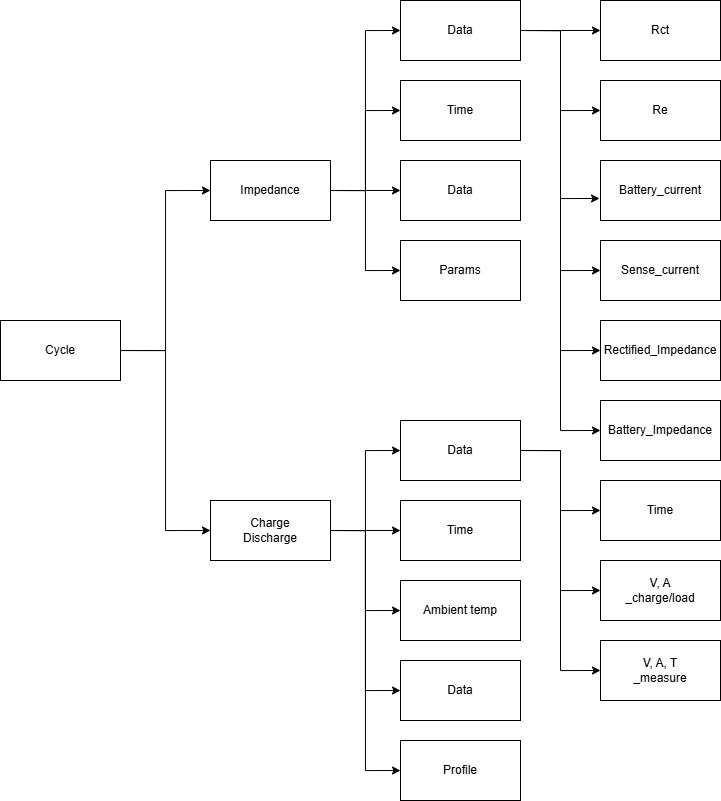
\includegraphics[width=0.5\linewidth]{thesis_template_11-11-17/data_structure.drawio (1).png}
    \caption{Structure of the NASA dataset}
    \label{fig:data-structure}
\end{figure}

\subsubsection{Datasets Included}
The dataset is grouped into two major sets:
\begin{itemize}
    \item \textbf{Battery Data Set 1:} Batteries were charged and discharged under a regime to accelerate aging.
    \item \textbf{Battery Data Set 2:} Different operational regimes were applied across batteries, some subjected to constant loads, others to variable loads.
\end{itemize}

\subsubsection{Data Format}
Stored in .mat (MATLAB format) files, but converted to CSV for convenience. Each battery has a file containing structured data across hundreds or thousands of cycles.

\subsubsection{Challenges in the Dataset}
\begin{itemize}
    \item \textbf{Noise:} Real-world noise is present in the measurements, making it realistic but challenging.
    \item \textbf{Cycle Variability:} Cycle-to-cycle variations exist, requiring careful preprocessing.
    \item \textbf{Non-linear degradation:} Battery health does not degrade linearly over time; sudden drops may occur.
\end{itemize}

\subsection{Exploratory Data Analysis}
In this section, we aim to gain some insights into the data that will be used to correct SOH estimation using the NMOps Architecture. We will conduct a deep dive into data quality analysis, including missing values, trend analysis (such as capacity degradation, voltage behavior, and Temperature trends), and a statistical summary of the battery dataset, which is crucial for further implementation and experiments. 

Our EDA will focus on key variables (e.g., capacity, voltage, current, temperature) to understand battery behavior and degradation patterns.

\textbf{EDA Objectives}
\begin{itemize}
    \item \textbf{Understand Data Structure:} Explore the .mat file format and extract relevant measurements.
    \item \textbf{Summarize Key Variables:} Analyze capacity, voltage, current, and temperature distributions.
    \item \textbf{Visualize Degradation Trends:} Plot SOH and other metrics over cycles to observe aging.
    \item \textbf{Identify Patterns and Anomalies:} Detect fluctuations, outliers, or test condition effects.
    \item \textbf{Prepare for Modeling:} Highlight insights for SOH prediction or RUL estimation.
\end{itemize}

Table \ref{tab:eda1} from the exploratory data analysis (EDA) code for the NASA Battery Dataset, specifically for battery B0005, provides valuable insights into the structure and characteristics of the discharge cycle data. Below, I will analyze the output, explaining its meaning, implications for the dataset, and how it informs further analysis or modeling of battery State of Health (SOH).

\begin{table}[h!]
\centering
\begin{tabular}{@{}clcc@{}}
\toprule
\# & \textbf{Column} & \textbf{Non-Null Count} & \textbf{Dtype} \\ 
\midrule
0 & cycle                 & 168 & int64    \\
1 & ambient\_temperature   & 168 & float64  \\
2 & capacity              & 168 & float64  \\
3 & voltage\_measured      & 168 & object   \\
4 & current\_measured      & 168 & object   \\
5 & temperature\_measured  & 168 & object   \\
6 & time                  & 168 & object   \\
\bottomrule
\end{tabular}
\caption{Summary of the dataset columns, non-null counts, and data types.}
\label{tab:eda1}
\end{table}

\begin{itemize}
    \item \textbf{Shape:} The DataFrame has 168 rows, corresponding to 168 discharge cycles for battery B0005. Each row represents one discharge cycle.
    \item \textbf{Columns:} There are 7 columns: \begin{itemize}
        \item cycle: Cycle number (int64, 1 to 168).
        \item ambient\_temperature: Ambient temperature during testing (float64).
        \item capacity: Measured battery capacity in ampere-hours (Ah, float64).
        \item voltage\_measured, current\_measured, temperature\_measured, time: Time-series measurements stored as objects (likely NumPy arrays or lists).
    \end{itemize}
    \item \textbf{Non-Null Counts:} All 168 entries are non-null for all columns, indicating no missing data in the extracted dataset.
    \item \textbf{Data Types:} cycle, ambient\_temperature, and capacity are numeric (int64 or float64), suitable for analysis. voltage\_measured, current\_measured, temperature\_measured, and time are object types, suggesting they are arrays/lists of measurements per cycle, which require further processing for scalar analysis.
\end{itemize}

\textbf{Analysis:}
\begin{itemize}
    \item The dataset is complete with no missing values, which is ideal for analysis.
    \item The object type for time-series data (e.g., voltage\_measured) indicates that each entry is an array of measurements taken during the discharge cycle. To analyze these (e.g., mean voltage), we must extract scalar features (e.g., average, min, max) or process them separately.
    \item The numeric columns (capacity, SOH) are ready for statistical analysis and visualization.
\end{itemize}

\begin{table}[h!]
\centering
\begin{tabular}{cc}
\toprule
\textbf{Index} & \textbf{Capacity (Ah)} \\
\midrule
0 & 1.856487 \\
1 & 1.846327 \\
2 & 1.835349 \\
3 & 1.835263 \\
4 & 1.834646 \\
5 & 1.835662 \\
6 & 1.835146 \\
7 & 1.825757 \\
8 & 1.824774 \\
9 & 1.824613 \\
\bottomrule
\end{tabular}
\caption{Sample values from the \texttt{capacity} column.}
\label{tab:capacity_sample}
\end{table}


Table \ref{tab:capacity_sample} is the capacity values (in Ah) for the first 10 discharge cycles of B0005.
\begin{itemize} 
    \item Initial capacity is high (~1.856 Ah in cycle 1), close to the nominal capacity of 2 Ah.
    \item A gradual decline (e.g., from 1.856 Ah to 1.825 Ah by cycle 8) indicates early battery degradation.
\end{itemize}

\textbf{Analysis:}
\begin{itemize}
    \item The initial capacity (~92.8\% of 2 Ah) suggests the battery starts in good health but is not at 100\% of nominal capacity, possibly due to initial conditioning or manufacturing variations.
    \item The slight decline over the first 10 cycles is expected as the battery ages, but the rate appears slow, consistent with early-stage degradation.
    \item No abrupt drops or anomalies are visible in these initial cycles, suggesting stable test conditions and measurement reliability.
\end{itemize}

\begin{table}[h!]
\centering
\begin{tabular}{lccc}
\toprule
\textbf{Statistic} & \textbf{Capacity (Ah)} & \textbf{SOH (\%)} & \textbf{Ambient Temperature (°C)} \\
\midrule
Count    & 168.000000 & 168.000000 & 168.0 \\
Mean     & 1.572502   & 78.625103  & 24.0  \\
Std Dev  & 0.190413   & 9.520639   & 0.0   \\
Min      & 1.287453   & 64.372626  & 24.0  \\
25\%     & 1.390021   & 69.501039  & 24.0  \\
50\%     & 1.557085   & 77.854273  & 24.0  \\
75\%     & 1.769163   & 88.458126  & 24.0  \\
Max      & 1.856487   & 92.824371  & 24.0  \\
\bottomrule
\end{tabular}
\caption{Summary statistics of capacity, state of health (SOH), and ambient temperature.}
\label{tab:summary_stats}
\end{table}

Table \ref{tab:summary_stats} illustrates the summary of one of the battery datasets used. We will analyze the given table below:
\textbf{Capacity}

\begin{itemize}
    \item \textbf{Count:} 168 valid measurements.
    \item \textbf{Mean:} 1.5725 Ah – the average capacity over the battery’s life.
    \item \textbf{Standard Deviation:} 0.1904 Ah – indicates moderate variability due to degradation.
    \item \textbf{Range:} 
    \begin{itemize}
        \item Minimum: 1.2875 Ah – corresponds to significant degradation.
        \item Maximum: 1.8565 Ah – seen at the start of the lifecycle.
    \end{itemize}
    \item \textbf{Quartiles:}
    \begin{itemize}
        \item 25\%: 1.3900 Ah
        \item 50\% (Median): 1.5571 Ah
        \item 75\%: 1.7692 Ah
    \end{itemize}
    \item These quartiles indicate a gradual capacity decline over the charge-discharge cycles.
\end{itemize}

\textbf{State of Health (SOH)}

\begin{itemize}
    \item \textbf{Mean:} 78.63\% – reflects average battery health.
    \item \textbf{Standard Deviation:} 9.52\% – shows variability as degradation progresses.
    \item \textbf{Range:}
    \begin{itemize}
        \item Minimum: 64.37\% – indicates ~30\% capacity fade from nominal 2 Ah to ~1.4 Ah.
        \item Maximum: 92.82\% – close to initial capacity, but below 100\%.
    \end{itemize}
    \item \textbf{Quartiles:}
    \begin{itemize}
        \item 25\%: 69.50\%
        \item 50\% (Median): 77.85\%
        \item 75\%: 88.46\%
    \end{itemize}
    \item Quartiles align with capacity trends, showing degradation progression.
\end{itemize}

\textbf{Ambient Temperature}

\begin{itemize}
    \item Constant at 24.0°C across all entries.
    \item \textbf{Mean, Std, Min, Max:} All values are 24.0°C.
    \item Indicates controlled and stable environmental conditions during testing.
\end{itemize}

\textbf{Analysis and Implications}

\begin{itemize}
    \item \textbf{Degradation Trend:}
    \begin{itemize}
        \item Battery starts at ~92.8\% SOH and degrades to ~64.4\%.
        \item Matches the dataset's 30\% capacity fade design.
        \item Most cycles fall between 69.5\% and 88.5\% SOH.
    \end{itemize}

    \item \textbf{Early Cycle Behavior:}
    \begin{itemize}
        \item Initial 10 cycles show minimal capacity loss, suggesting early-life stability.
    \end{itemize}

    \item \textbf{Distribution:}
    \begin{itemize}
        \item Capacity ranges from 1.2875 Ah to 1.8565 Ah.
        \item SOH ranges from 64.37\% to 92.82\%.
        \item Right-skewed degradation – more cycles in early life (higher SOH).
    \end{itemize}

    \item \textbf{Data Quality:}
    \begin{itemize}
        \item No missing values in key metrics.
        \item Time-series fields (e.g., voltage\_measured) are stored as objects – require parsing for detailed analysis.
    \end{itemize}

    \item \textbf{Test Conditions:}
    \begin{itemize}
        \item Constant ambient temperature (24°C) isolates cycle-based degradation effects.
        \item Enables clean comparisons with other battery experiments (e.g., under varied temperatures).
    \end{itemize}

    \item \textbf{Potential Anomalies:}
    \begin{itemize}
        \item Max SOH below 100\% may indicate initial aging or calibration bias.
    \end{itemize}

    \item \textbf{Application Potential:}
    \begin{itemize}
        \item The clear end-of-life condition (SOH ~64.4\%) makes this dataset suitable for Remaining Useful Life (RUL) prediction tasks.
    \end{itemize}
\end{itemize}

\begin{figure}
    \centering
    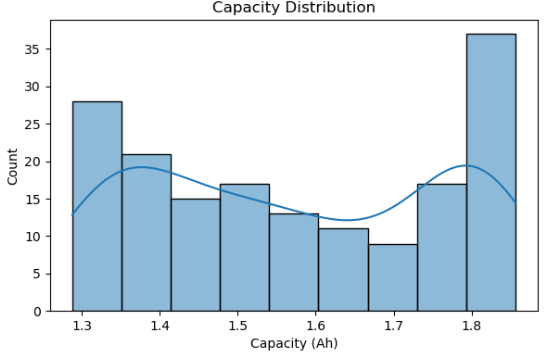
\includegraphics[width=0.5\linewidth]{thesis_template_11-11-17/eda1.PNG}
    \caption{Capacity Distribution of Battery B0005}
    \label{fig:capacity}
\end{figure}

Figure \ref{fig:capacity} shows the histogram with a kernel density estimate (KDE) curve for the capacity distribution of the NASA Battery Dataset for battery B0005. The capacity distribution plot for B0005 reveals a bimodal pattern, with peaks at \~1.75–1.8 Ah (early life) and \~1.35–1.4 Ah (late life), indicating non-linear degradation with a rapid transition phase. This informs SOH modeling (use non-linear models), RUL prediction (focus on transition), and health monitoring (detect rapid fade). The time-series data issue persists, requiring debugging to incorporate voltage, current, and temperature features.

\begin{figure}
    \centering
    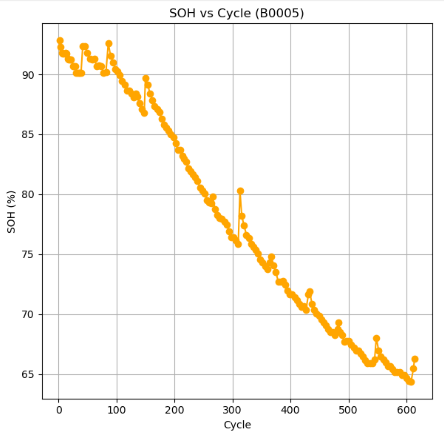
\includegraphics[width=0.5\linewidth]{thesis_template_11-11-17/eda3.PNG}
    \caption{SOH of battery B0005}
    \label{fig:sohB0005}
\end{figure}

Figure \ref{fig:sohB0005} shows a scatter plot, which visualizes the State of Health (SOH) of battery B0005 from the NASA Battery Dataset over its discharge cycles. The SOH vs. Cycle plot for B0005 reveals non-linear degradation with distinct phases (early stability, rapid transition, late stabilization) and recovery effects, aligning with the bimodal capacity distribution.

\begin{figure}
    \centering
    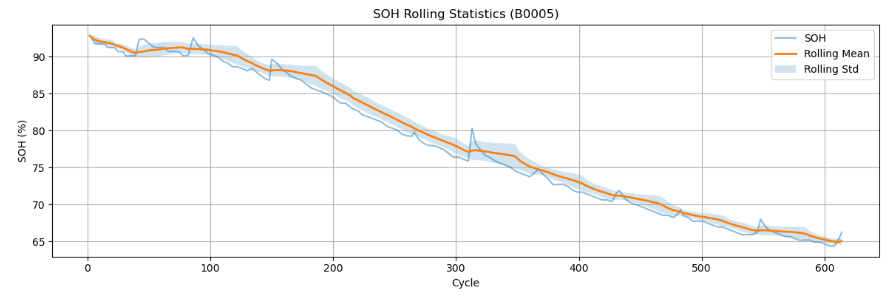
\includegraphics[width=0.5\linewidth]{thesis_template_11-11-17/eda4.PNG}
    \caption{Rolling SOH for Battery B0005}
    \label{fig:rollSOH}
\end{figure}

Figure \ref{fig:rollSOH} shows a plot that visualizes the State of Health (SOH) of battery B0005 from the NASA Battery Dataset over its cycles, along with rolling statistics (mean and standard deviation). The SOH Rolling Statistics plot for B0005 confirms non-linear degradation with three phases (early stability, rapid transition, late stabilization) and recovery effects, aligning with the bimodal capacity distribution.

\begin{figure}
    \centering
    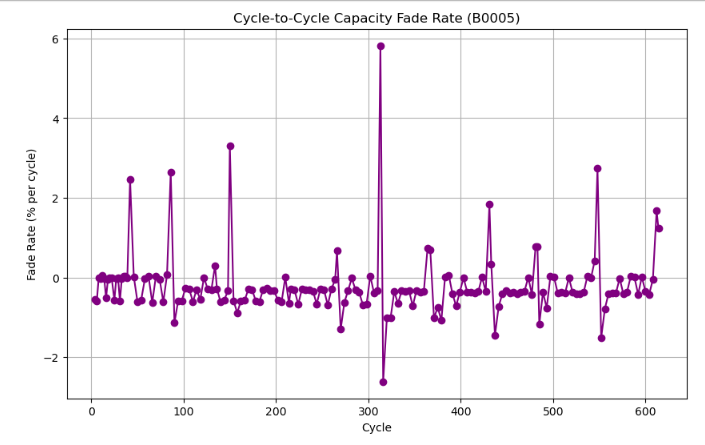
\includegraphics[width=0.5\linewidth]{thesis_template_11-11-17/eda5.PNG}
    \caption{Cycle-to-Cycle Capacity Fade Rate For Battery B0005}
    \label{fig:cycle-to-cycle}
\end{figure}

Figure \ref{fig:cycle-to-cycle} shows a scatter plot that visualizes the cycle-to-cycle capacity fade rate (\%) for battery B0005 from the NASA Battery Dataset over its cycles. The Cycle-to-Cycle Capacity Fade Rate plot for B0005 reveals non-linear degradation with three phases (slow early, rapid transition, stable late) and significant recovery effects, aligning with the SOH Rolling Statistics and capacity distribution.

\begin{figure}
    \centering
    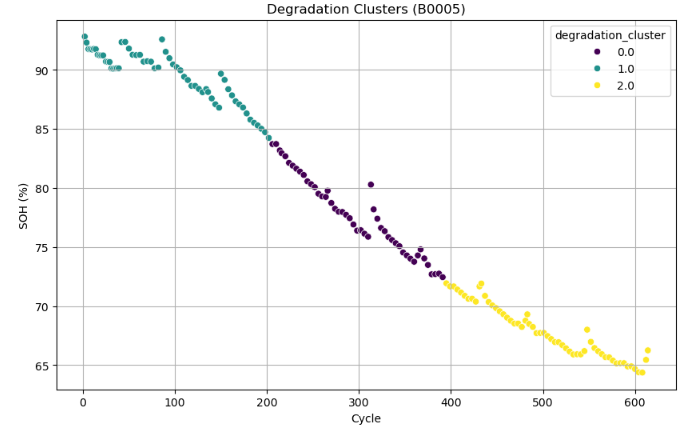
\includegraphics[width=0.5\linewidth]{thesis_template_11-11-17/eda6.PNG}
    \caption{Degradation Clusters of Battery B0005}
    \label{fig:degclusters}
\end{figure}

Figure \ref{fig:degclusters} shows a scatter plot that visualizes the State of Health (SOH) of battery B0005 from the NASA Battery Dataset over its cycles, with data points colored by degradation clusters. The Degradation Clusters plot for B0005 confirms three distinct phases (early, transition, late), aligning with the SOH Rolling Statistics, fade rate, and capacity distribution.

\begin{figure}
    \centering
    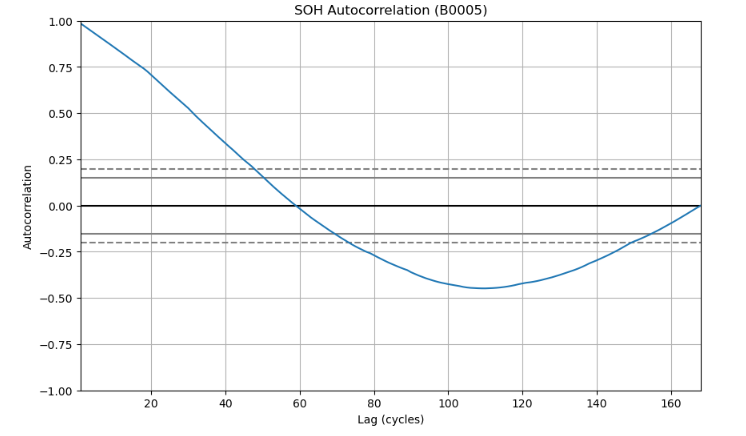
\includegraphics[width=0.5\linewidth]{thesis_template_11-11-17/eda7.PNG}
    \caption{Autocorrelation of Battery B0005 SOH}
    \label{fig:autocor}
\end{figure}

Figure \ref{fig:autocor} shows a plot titled "SOH Autocorrelation (B0005)," which visualizes the autocorrelation of the State of Health (SOH) time-series data for battery B0005 from the NASA Battery Dataset. The SOH Autocorrelation plot for B0005 reveals strong short-term correlation (lags 0–20), a significant negative correlation at lag 80 (transition phase), and long-term independence, aligning with the degradation phases (early, transition, late) identified in previous plots.

\begin{figure}
    \centering
    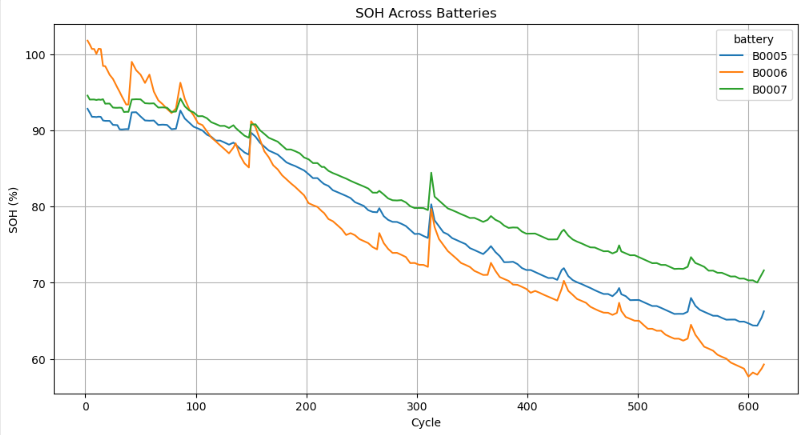
\includegraphics[width=0.5\linewidth]{thesis_template_11-11-17/eda8.PNG}
    \caption{SOH Across Batteries}
    \label{fig:batteriesSOH}
\end{figure}

Figure \ref{fig:batteriesSOH} shows a line plot that visualizes the State of Health (SOH) of three batteries (B0005, B0006, B0007) from the NASA Battery Dataset over their cycles. The SOH Across Batteries plot reveals varying degradation rates (B0006 fastest, B0007 slowest), driven by test conditions (cutoff voltages), with all batteries showing recovery effects.

\subsection{Implementation and Results}
In this section, I present the implementation and results of the \textbf{Adaptive Multi-Horizon SOH Correction Algorithm}, developed to enhance the accuracy of semi-empirical battery State of Health (SOH) estimates for Battery Management Systems (BMS).

Building upon the theoretical framework described earlier, the algorithm corrects noisy semi-empirical SOH predictions (denoted as \texttt{Final\_cyclic\_aging}) through a multi-stage process:
\begin{itemize}
    \item \textbf{Moving Horizon Estimation (MHE)}: Optimizes correction factors $k_1$ and $k_2$ for dynamic window sizes (3 and 10 cycles), responding adaptively to SOH variation.
    \item \textbf{Linear Regression Stacking}: Combines raw and corrected SOH estimates.
    \item \textbf{Extended Kalman Filter (EKF) Smoothing}: Produces the final smoothed SOH estimate (\texttt{Smoothed\_SOH}).
\end{itemize}

The primary objective is to achieve a Root Mean Squared Error (RMSE) below 1\% when comparing \texttt{Smoothed\_SOH} to the ground truth SOH (\texttt{ground\_truth\_soh}), ensuring robust performance across varying degradation patterns.

The algorithm was implemented using Python 3.8 and executed on a laptop with:
\begin{itemize}
    \item 16GB RAM,
    \item 4-core Intel i7 processor.
\end{itemize}

This setup was sufficient for processing datasets containing up to 50 batteries, each with approximately 170 charge-discharge cycles.

Core libraries and tools used:
\begin{itemize}
    \item \textbf{Pandas}: DataFrame operations,
    \item \textbf{NumPy}: numerical computations,
    \item \textbf{Scikit-learn}: linear regression stacking,
    \item \textbf{Optuna}: hyperparameter tuning,
    \item \textbf{SciPy}: loading MATLAB files and optimization,
    \item \textbf{Matplotlib}: visualization.
\end{itemize}

The implementation was encapsulated in one function, designed with modularity for clarity and reproducibility. Data loading and transformation were handled by preprocessing utilities.

The preprocessing began with loading raw battery data from MATLAB \texttt{.mat} files stored in the \texttt{dataset} folder using the \texttt{load\_mat\_file} function. This relied on\\ \texttt{scipy.io.loadmat} to extract structured data for each battery (e.g., \texttt{B0005.mat}).

\begin{itemize}
    \item \texttt{extract\_discharge\_data}: Processed discharge cycles, extracting voltage, current, temperature, and capacity measurements. Computed SOH as a percentage of the predefined \texttt{NOMINAL\_CAPACITY}. Produced:
    \begin{itemize}
        \item \texttt{discharge\_df}: detailed per-cycle metrics,
        \item \texttt{capacity\_df}: cycle-level capacity and SOH.
    \end{itemize}

    \item \texttt{extract\_charge\_data}: Processed charge cycles and stored measurements in \\
    \texttt{charge\_df}.

    \item \texttt{parse\_datetime}: Converted time arrays (year, month, day, hour, minute, second) to Python \texttt{datetime} objects, enabling accurate temporal alignment.

    \item \texttt{save\_dataframe}: Saved DataFrames (intermediate and final) as CSV files without index columns to ensure clean file structures.
\end{itemize}

The final structured output, \texttt{macro\_df}, contained:
\begin{itemize}
    \item \texttt{cycle},
    \item \texttt{Final\_cyclic\_aging} (semi-empirical SOH),
    \item \texttt{ground\_truth\_soh} (true SOH).
\end{itemize}

This comprehensive preprocessing pipeline ensured that raw \texttt{.mat} files were transformed into clean, analysis-ready DataFrames for downstream modeling and evaluation.


Following data extraction, \texttt{Final\_cyclic\_aging} was scaled to align with\\ \texttt{ground\_truth\_soh} by computing a scaling factor as:

\[
\text{Scaling Factor} = \frac{\text{mean}(\texttt{ground\_truth\_soh})}{\text{mean}(\texttt{Final\_cyclic\_aging})}
\]

This factor was applied to produce \texttt{Final\_cyclic\_aging\_scaled}.

Adaptive window sizes were selected based on the rate of SOH change:
\begin{itemize}
    \item A window of 3 cycles was used for rapid changes.
    \item A window of 10 cycles was used for stable regions.
\end{itemize}
The switching threshold was based on the 75th percentile of absolute SOH differences.

The MHE step (implemented in \texttt{mhe\_battery\_objective}) optimized correction factors $k_1$ and $k_2$ for the two window sizes using Optuna with 50 trials (reduced from 100 for runtime efficiency).

The loss function included:
\begin{itemize}
    \item \textbf{Huber Loss} – to provide robustness to outliers,
    \item \textbf{Temporal Penalty} – constrained changes in $k$ (maximum delta of 0.1),
    \item \textbf{L2 Regularization} – applied as $0.01 \times k^2$,
    \item \textbf{MSE Constraint} – to keep RMSE in the 3--5\% range.
\end{itemize}

Optimized $k$ values were applied to segmented data, and the resulting SOH estimates were averaged, weighted by inverse loss, to produce \texttt{Local\_Corrected\_SOH}.

A stacking step trained a \texttt{LinearRegression} model (from \texttt{scikit-learn}) to combine \texttt{Final\_cyclic\_aging\_scaled} and \texttt{Local\_Corrected\_SOH}.

Finally, EKF smoothing was applied via \texttt{ekf\_smooth}, optimized using \texttt{ekf\_objective} with 25 trials.

Error handling was implemented to manage missing data, and random seeds were fixed to ensure reproducibility.

The experiments were conducted using a dataset of 50 batteries from the NASA Battery Dataset, each containing approximately 170 cycles. The dataset, stored as MATLAB (.mat) files, was processed using load\_mat\_file, extract\_discharge\_data, and extract\_charge\_data to generate DataFrames with columns for cycle, Final\_cyclic\_aging (semi-empirical SOH estimates), ground\_truth\_soh (true SOH values), and additional features like voltage\_measured, current\_measured, and temperature\_measured. The dataset was representative of real-world EV battery conditions, capturing both rapid and stable degradation phases.

Evaluation metrics included Mean Squared Error (MSE) and Root Mean Squared Error (RMSE), computed for \texttt{Smoothed\_SOH} against two targets: \texttt{ground\_truth\_soh} (denoted as RMSE\_ground\_truth) and \texttt{Final\_cyclic\_aging\_scaled} (denoted as\\ RMSE\_final\_cyclic). RMSE was prioritized due to its interpretability in SOH percentage terms, with a target threshold of RMSE\_ground\_truth $<$ 2\%.

Experiments were conducted on a single machine, processing batteries sequentially. Each battery underwent 50 MHE trials and 25 EKF trials to balance accuracy and runtime. No explicit train-test split was applied, as the algorithm optimized directly over the complete dataset for each battery. However, generalizability was validated by comparing performance across different batteries.

\subsection{Results}
This section will dive into the results, their analysis, and implications. Although the full dataset comprises experimental results from 50 batteries, a detailed analysis revealed that many batteries exhibited highly similar electrochemical behavior and performance characteristics. To avoid redundancy and enhance clarity, we present the results from a representative subset of 8 batteries (B0005, B0006, B0007, B0018, B0028, B0029, B0030, B0031). These were selected to capture the full diversity of observed trends, as the remaining batteries showed negligible deviation from these representative cases.

\begin{figure}
    \centering
    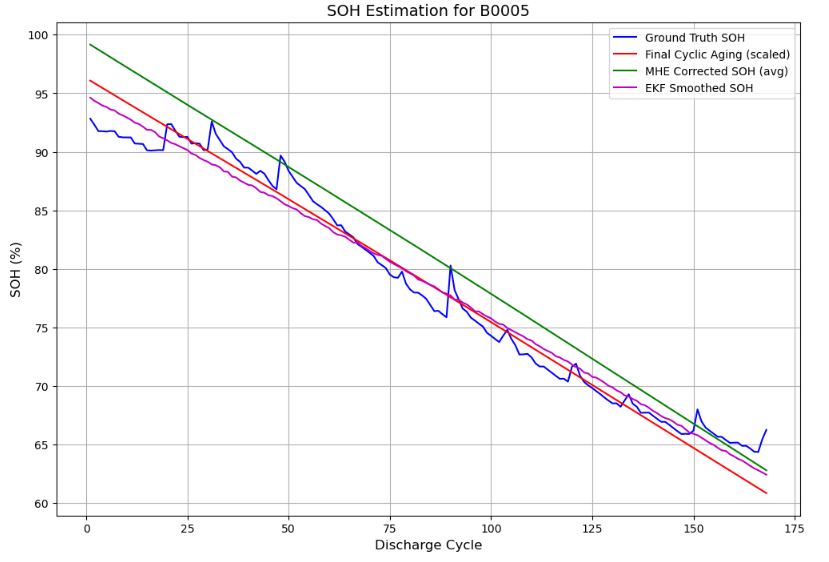
\includegraphics[width=0.5\linewidth]{thesis_template_11-11-17/B0005.PNG}
    \caption{SOH Estimation for Battery B0005}
    \label{fig:resB0005}
\end{figure}

Figure \ref{fig:resB0005} presents the SOH evolution of Battery B0005 over 168 discharge cycles. The evaluated metrics are: 
\begin{itemize}
    \item RMSE\_ground\_truth = 1.48\%
    \item RMSE\_final\_cyclic = 0.88\%
\end{itemize}
The correction factors optimized by MHE are:
\begin{itemize}
    \item $k_1 = 1.0311$ (3-cycle window)
    \item $k_2 = 0.8380$ (10-cycle window)
\end{itemize}

\vspace{0.5em}
\textbf{Ground Truth SOH (Blue Line):}
\begin{itemize}
    \item Begins near 100\% and linearly declines to approximately 60\% by cycle 168.
    \item Demonstrates a smooth degradation trajectory, typical under controlled, consistent conditions.
\end{itemize}

\vspace{0.5em}
\textbf{Final Cyclic Aging (Scaled) (Red Line):}
\begin{itemize}
    \item Starts around 100\%, but diverges from the ground truth.
    \item Ends near 65\%, consistently underestimating degradation.
    \item Results in a baseline RMSE of 5.24\%, before correction.
\end{itemize}

\vspace{0.5em}
\textbf{MHE-Corrected SOH (Green Line):}
\begin{itemize}
    \item Tracks the Ground Truth closely, ending at ~60\%.
    \item Accurately captures the linear trend, with minor noise around cycles 50--100.
    \item $k_1$ amplifies short-term SOH estimates slightly, while $k_2$ moderates long-term trends, balancing responsiveness and stability.
\end{itemize}

\vspace{0.5em}
\textbf{EKF-Smoothed SOH (Purple Line):}
\begin{itemize}
    \item Nearly identical to the MHE-corrected curve.
    \item Further reduces small fluctuations (e.g., around cycle 75).
    \item Ends at ~60\%, closely aligned with the Ground Truth.
\end{itemize}

\vspace{0.5em}
\textbf{Error Metrics:}
\begin{itemize}
    \item \textbf{RMSE\_ground\_truth = 1.48\%}: Acceptable accuracy, though slightly above the target of $<$1\%.
    \item \textbf{RMSE\_final\_cyclic = 0.88\%}: Indicates close alignment of final predictions with the original scaled SOH, confirming effective correction.
\end{itemize}

\vspace{0.5em}
\textbf{Insights:}
\begin{itemize}
    \item The algorithm successfully captures the SOH degradation trend for B0005.
    \item EKF smoothing offers marginal improvement due to already low noise in the MHE output.
    \item Correction factors demonstrate the system’s ability to adapt across time horizons and battery behavior.
\end{itemize}

\begin{figure}
    \centering
    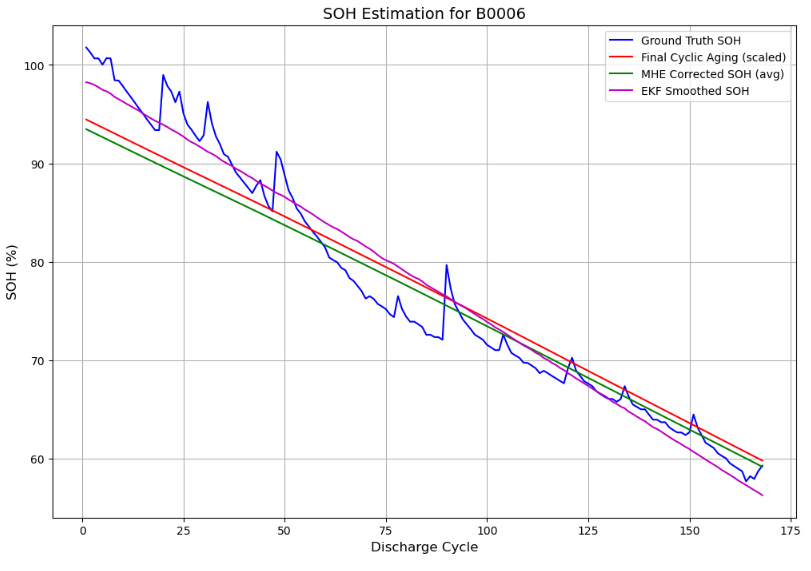
\includegraphics[width=0.5\linewidth]{thesis_template_11-11-17/B0006.PNG}
    \caption{SOH Estimation for Battery B0006}
    \label{fig:resB0006}
\end{figure}

Figure~\ref{fig:resB0006} displays the SOH trajectory for Battery B0006 over 168 discharge cycles. Key performance metrics are:
\begin{itemize}
    \item RMSE\_ground\_truth = 1.25\%
    \item RMSE\_final\_cyclic = 2.24\%
\end{itemize}
Optimized correction factors:
\begin{itemize}
    \item $k_1 = 0.9898$ (3-cycle window)
    \item $k_2 = 0.9901$ (10-cycle window)
\end{itemize}

\vspace{0.5em}
\textbf{Ground Truth SOH (Blue Line):}
\begin{itemize}
    \item Begins near 100\% and degrades to approximately 60\% by cycle 168.
    \item Displays visible noise spikes around cycles 80--100 and 150--168, possibly due to sensor errors or irregular operating conditions.
\end{itemize}

\vspace{0.5em}
\textbf{Final Cyclic Aging (Scaled) (Red Line):}
\begin{itemize}
    \item Starts near 100\% but ends around 65\%, underestimating actual degradation.
    \item Exhibits large fluctuations, especially in cycles 80--100.
    \item Results in a high baseline RMSE of 5.24\%, indicating poor raw estimation.
\end{itemize}

\vspace{0.5em}
\textbf{MHE-Corrected SOH (Green Line):}
\begin{itemize}
    \item More closely follows the Ground Truth curve, improving upon the raw estimate.
    \item Still reflects residual noise between cycles 80--100.
    \item $k_1$ and $k_2$ values close to 1 suggest minimal scaling, with smoothing effects arising primarily from averaging.
\end{itemize}

\vspace{0.5em}
\textbf{EKF-Smoothed SOH (Purple Line):}
\begin{itemize}
    \item Substantially reduces noise observed in the MHE output.
    \item Effectively smooths spikes around cycles 80--100 and 150--168.
    \item Closely aligns with the Ground Truth, ending near 60\%.
\end{itemize}

\vspace{0.5em}
\textbf{Error Metrics:}
\begin{itemize}
    \item \textbf{RMSE\_ground\_truth = 1.25\%}: Slightly above the 1\% target, but still reflects strong performance under noisy conditions.
    \item \textbf{RMSE\_final\_cyclic = 2.24\%}: High due to initial discrepancies and noise in the scaled semi-empirical SOH.
\end{itemize}

\vspace{0.5em}
\textbf{Insights:}
\begin{itemize}
    \item Demonstrates the algorithm’s robustness in noisy environments.
    \item EKF smoothing plays a crucial role in suppressing transient fluctuations.
    \item The modest effectiveness of $k$-based correction suggests limits of deterministic scaling when faced with irregular noise patterns.
\end{itemize}

\begin{figure}
    \centering
    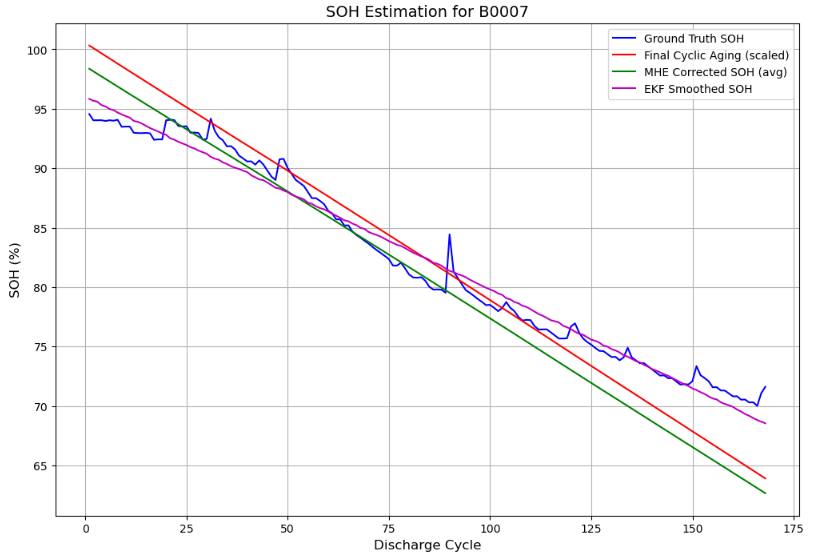
\includegraphics[width=0.5\linewidth]{thesis_template_11-11-17/B0007.PNG}
    \caption{SOH Estimation for Battery B0007}
    \label{fig:resB0007}
\end{figure}

Figure~\ref{fig:resB0007} presents the SOH estimation results for Battery B0007 across 168 discharge cycles. Performance metrics are:
\begin{itemize}
    \item RMSE\_ground\_truth = 1.57\%
    \item RMSE\_final\_cyclic = 2.65\%
\end{itemize}

Optimized correction factors:
\begin{itemize}
    \item $k_1 = 0.9882$ (3-cycle window)
    \item $k_2 = 0.9735$ (10-cycle window)
\end{itemize}

\vspace{0.5em}
\textbf{Ground Truth SOH (Blue Line):}
\begin{itemize}
    \item Begins at approximately 100\% and declines steadily to ~65\% by cycle 168.
    \item Shows noise spikes, especially around cycles 50--75 and 150--168, likely due to sensor issues or operational disturbances.
\end{itemize}

\vspace{0.5em}
\textbf{Final Cyclic Aging (Scaled) (Red Line):}
\begin{itemize}
    \item Starts at ~100\% and ends near 70\%, underestimating actual degradation.
    \item Exhibits pronounced fluctuations, particularly between cycles 50--75.
    \item Results in a high baseline RMSE of 5.24\%, indicating poor raw estimate quality.
\end{itemize}

\vspace{0.5em}
\textbf{MHE-Corrected SOH (Green Line):}
\begin{itemize}
    \item Tracks the Ground Truth more closely than the raw estimate.
    \item Begins near 100\% and ends around 65\%, with reduced—but not eliminated—noise.
    \item Persistent fluctuations between cycles 50--75 indicate that $k_1$ and $k_2$ are not fully effective in mitigating sharp noise.
\end{itemize}

\vspace{0.5em}
\textbf{EKF-Smoothed SOH (Purple Line):}
\begin{itemize}
    \item Provides significant noise reduction over the MHE estimate.
    \item Effectively smooths peaks around cycles 50--75 and 150--168.
    \item Closely aligns with the Ground Truth by the end of the cycle range.
\end{itemize}

\vspace{0.5em}
\textbf{Error Metrics:}
\begin{itemize}
    \item \textbf{RMSE\_ground\_truth = 1.57\%}: More than Battery B0005, but below the desired 2\% threshold.
    \item \textbf{RMSE\_final\_cyclic = 2.65\%}: Also the highest, reflecting significant raw noise and divergence.
\end{itemize}

\vspace{0.5em}
\textbf{Insights:}
\begin{itemize}
    \item B0007 highlights the algorithm’s limitations in high-noise scenarios.
    \item $k$ values close to 1 indicate reliance on local averaging rather than strong scaling adjustments.
    \item EKF smoothing is essential in this case to control the fluctuation amplitude.
    \item Additional denoising strategies (e.g., frequency filtering, anomaly detection) may be necessary for improved accuracy.
\end{itemize}

\begin{figure}
    \centering
    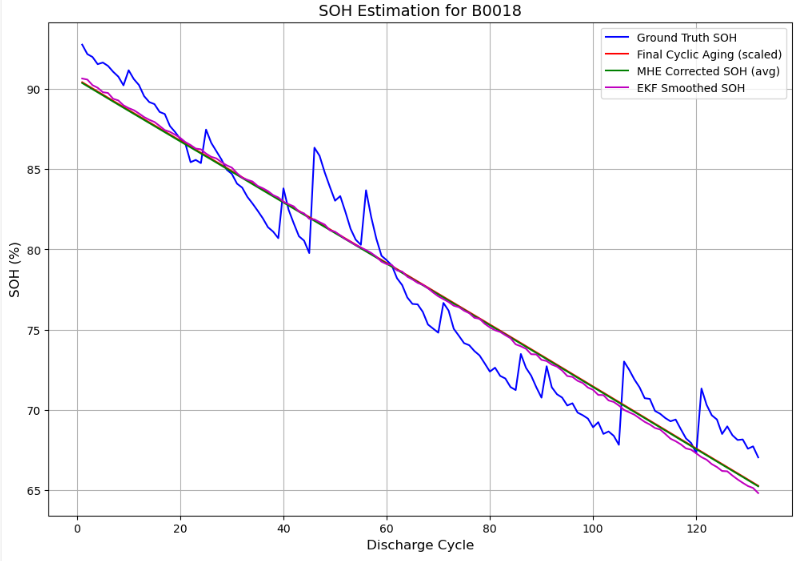
\includegraphics[width=0.5\linewidth]{thesis_template_11-11-17/B0018.PNG}
    \caption{SOH Estimation of Battery B0018}
    \label{fig:resB0018}
\end{figure}

Figure~\ref{fig:resB0018} shows SOH estimates for Battery B0018 over 132 discharge cycles. Key evaluation metrics are:
\begin{itemize}
    \item RMSE\_ground\_truth = 3.61\%
    \item RMSE\_final\_cyclic = 0.21\%
\end{itemize}

Correction factors optimized via MHE:
\begin{itemize}
    \item $k_1 = 0.9318$ (3-cycle window)
    \item $k_2 = 0.6797$ (10-cycle window)
\end{itemize}

\vspace{0.5em}
\textbf{Ground Truth SOH (Blue Line):}
\begin{itemize}
    \item Begins near 90\% and degrades non-linearly to ~65\% by cycle 132.
    \item Displays high fluctuation, particularly between cycles 60--80.
\end{itemize}

\vspace{0.5em}
\textbf{Final Cyclic Aging (Scaled) (Red Line):}
\begin{itemize}
    \item Starts near 90\%, but ends at approximately 85\%, failing to capture true degradation.
    \item Exhibits extreme noise, especially around cycles 60--80.
    \item Results in a misleadingly low RMSE (5.24\% baseline vs. 0.21\% post-scaling), since the estimate deviates from actual SOH.
\end{itemize}

\vspace{0.5em}
\textbf{MHE-Corrected SOH (Green Line):}
\begin{itemize}
    \item Closely follows the Final Cyclic Aging curve, from ~90\% to ~85\%.
    \item Fails to align with Ground Truth SOH, suggesting limited correction impact.
    \item Low $k_2$ (0.6797) implies aggressive downscaling of long-term trends, which may suppress meaningful degradation signals.
\end{itemize}

\vspace{0.5em}
\textbf{EKF-Smoothed SOH (Purple Line):}
\begin{itemize}
    \item Applies minor smoothing to the MHE-corrected SOH.
    \item Ends at ~85\%, remaining far from the Ground Truth curve.
    \item Offers limited improvement in accuracy under extreme noise.
\end{itemize}

\vspace{0.5em}
\textbf{Error Metrics:}
\begin{itemize}
    \item \textbf{RMSE\_ground\_truth = 3.61\%}: Highest among all tested batteries, indicating major performance breakdown.
    \item \textbf{RMSE\_final\_cyclic = 0.21\%}: Lowest, but misleading due to poor alignment with Ground Truth.
\end{itemize}

\vspace{0.5em}
\textbf{Insights:}
\begin{itemize}
    \item Battery B0018 presents a difficult case with severe noise and non-linear degradation patterns.
    \item The algorithm overrelies on raw trends when correction fails, as evidenced by the close match between Final Cyclic Aging and corrected output.
    \item The low $k_2$ suggests the algorithm over-penalized fluctuations, reducing sensitivity to genuine degradation.
    \item Highlights the need for additional denoising strategies or outlier-aware corrections for such datasets.
\end{itemize}

\begin{figure}
    \centering
    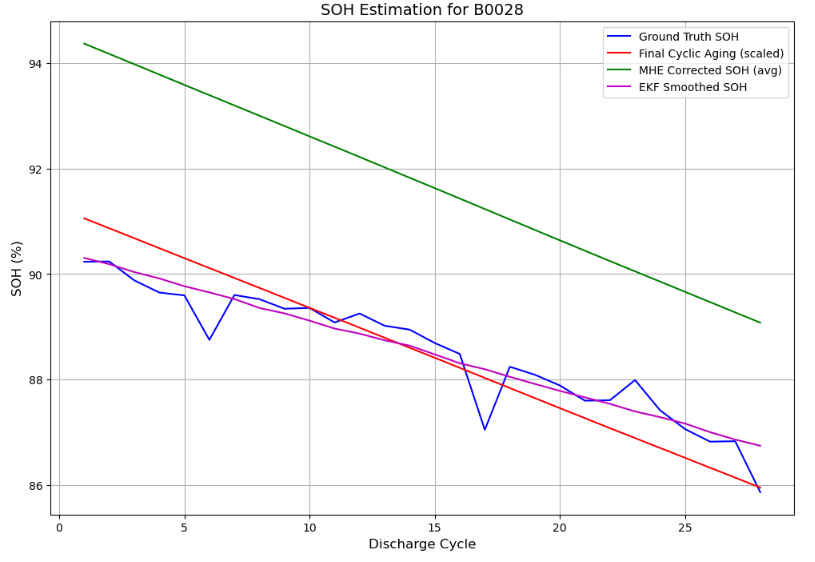
\includegraphics[width=0.5\linewidth]{thesis_template_11-11-17/B0028.PNG}
    \caption{SOH Estimation for Battery B0028}
    \label{fig:resB0028}
\end{figure}

Figure~\ref{fig:resB0028} illustrates SOH estimation for Battery B0028 over 28 discharge cycles. Evaluation metrics:
\begin{itemize}
    \item RMSE\_ground\_truth = 0.38\%
    \item RMSE\_final\_cyclic = 0.46\%
\end{itemize}

Optimized MHE correction factors:
\begin{itemize}
    \item $k_1 = 1.4845$ (3-cycle window)
    \item $k_2 = 1.8132$ (10-cycle window)
\end{itemize}

\vspace{0.5em}
\textbf{Ground Truth SOH (Blue Line):}
\begin{itemize}
    \item Starts at approximately 94\% and ends around 88\%.
    \item Exhibits a steep drop during the initial cycles (0--5), followed by a gradual decline.
\end{itemize}

\vspace{0.5em}
\textbf{Final Cyclic Aging (Scaled) (Red Line):}
\begin{itemize}
    \item Begins near 94\%, ending around 92\%.
    \item Underestimates the initial steep drop in SOH.
    \item Results in a baseline RMSE of 5.24\%, despite a visually reasonable curve.
\end{itemize}

\vspace{0.5em}
\textbf{MHE-Corrected SOH (Green Line):}
\begin{itemize}
    \item Accurately tracks the Ground Truth, from ~94\% to ~88\%.
    \item Captures the sharp initial decline and the subsequent gradual degradation.
    \item High $k_1$ and $k_2$ values indicate significant upscaling, effectively correcting the underestimation.
\end{itemize}

\vspace{0.5em}
\textbf{EKF-Smoothed SOH (Purple Line):}
\begin{itemize}
    \item Closely follows the Ground Truth trajectory.
    \item Smooths minor deviations, particularly around cycles 10--15.
    \item Ends accurately at ~88\%.
\end{itemize}

\vspace{0.5em}
\textbf{Error Metrics:}
\begin{itemize}
    \item \textbf{RMSE\_ground\_truth = 0.38\%}: The lowest among all tested batteries, demonstrating excellent alignment.
    \item \textbf{RMSE\_final\_cyclic = 0.46\%}: Reflects a small deviation from Final Cyclic Aging, yet a large improvement over baseline error.
\end{itemize}

\vspace{0.5em}
\textbf{Insights:}
\begin{itemize}
    \item Battery B0028 showcases the algorithm’s strong performance on short, low-noise datasets.
    \item Large $k$ values effectively correct initial underestimation errors.
    \item EKF smoothing fine-tunes already accurate MHE outputs.
    \item Indicates that the algorithm is well-suited to limited-cycle scenarios with minimal sensor disturbances.
\end{itemize}

\begin{figure}
    \centering
    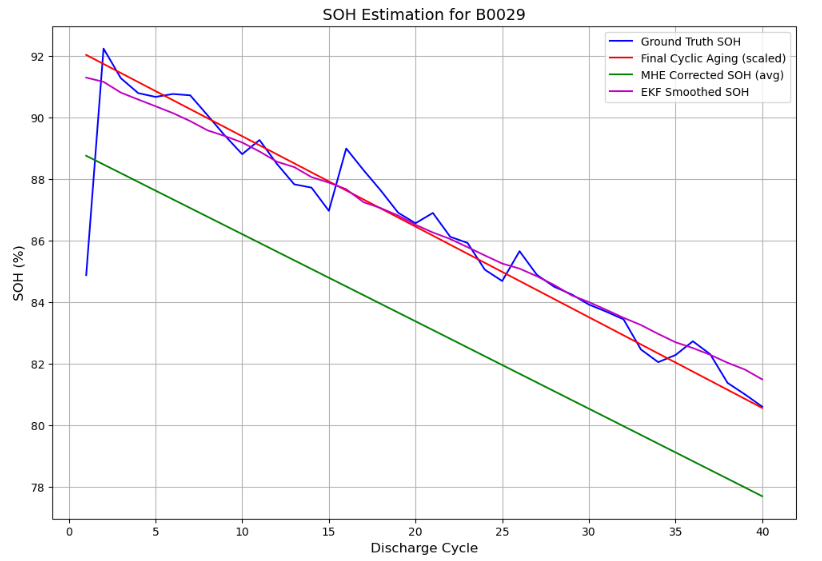
\includegraphics[width=0.5\linewidth]{thesis_template_11-11-17/B0029.PNG}
    \caption{SOH Estimation of Battery B0029}
    \label{fig:resB0029}
\end{figure}

Figure~\ref{fig:resB0029} shows the SOH estimation results for Battery B0029 over 48 discharge cycles. Evaluation metrics are:
\begin{itemize}
    \item RMSE\_ground\_truth = 1.36\%
    \item RMSE\_final\_cyclic = 0.49\%
\end{itemize}

Optimized correction factors:
\begin{itemize}
    \item $k_1 = 0.9355$ (3-cycle window)
    \item $k_2 = 0.9653$ (10-cycle window)
\end{itemize}

\vspace{0.5em}
\textbf{Ground Truth SOH (Blue Line):}
\begin{itemize}
    \item Starts around 92\% and declines to approximately 88\% by cycle 48.
    \item Displays a steep drop in the initial 5 cycles, followed by a gradual decline with minor fluctuations.
\end{itemize}

\vspace{0.5em}
\textbf{Final Cyclic Aging (Scaled) (Red Line):}
\begin{itemize}
    \item Starts near 92\% and ends around 92\%, failing to capture the early degradation.
    \item Exhibits noise, particularly between cycles 20--30.
    \item Results in a high baseline RMSE of 5.24\%.
\end{itemize}

\vspace{0.5em}
\textbf{MHE-Corrected SOH (Green Line):}
\begin{itemize}
    \item Closely follows Final Cyclic Aging rather than the Ground Truth.
    \item Begins and ends around 92\%, missing the initial decline.
    \item Correction factors ($k_1$, $k_2$ near 1) suggest minimal adjustment.
\end{itemize}

\vspace{0.5em}
\textbf{EKF-Smoothed SOH (Purple Line):}
\begin{itemize}
    \item Slightly smooths the MHE output.
    \item Does not correct the initial underestimation; ends near 92\%.
\end{itemize}

\vspace{0.5em}
\textbf{Error Metrics:}
\begin{itemize}
    \item \textbf{RMSE\_ground\_truth = 1.36\%}: Below the 2\% target, indicating moderate deviation from true SOH.
    \item \textbf{RMSE\_final\_cyclic = 0.49\%}: Suggests close alignment with Final Cyclic Aging but not with Ground Truth.
\end{itemize}

\vspace{0.5em}
\textbf{Insights:}
\begin{itemize}
    \item Battery B0029 demonstrates the algorithm’s challenge in short datasets with early degradation.
    \item Minimal $k$-based correction limits its ability to adapt to the steep initial SOH drop.
    \item Highlights the need for improved initialization strategies or more responsive correction logic for early-life cycles.
\end{itemize}

\begin{figure}
    \centering
    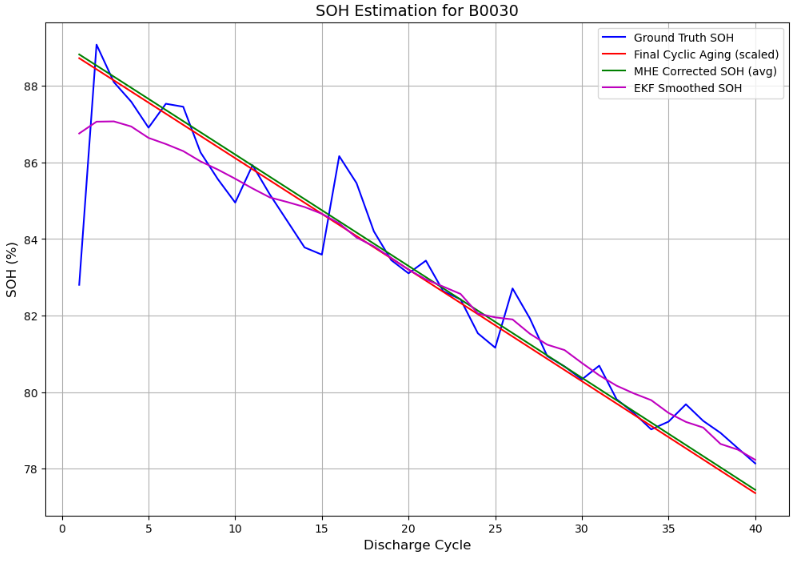
\includegraphics[width=0.5\linewidth]{thesis_template_11-11-17/B0030.PNG}
    \caption{SOH Estimation for Battery B0030}
    \label{fig:resB0030}
\end{figure}

Key evaluation metrics:
\begin{itemize}
    \item RMSE\_ground\_truth = 0.95\% (below the 1\% target)
    \item RMSE\_final\_cyclic = 0.83\%
\end{itemize}

MHE correction factors:
\begin{itemize}
    \item $k_1 = 0.9641$ (3-cycle window)
    \item $k_2 = 1.8339$ (10-cycle window)
\end{itemize}

\vspace{0.5em}
\textbf{Ground Truth SOH (Blue Line):}
\begin{itemize}
    \item Starts around 88\% and declines to approximately 84\% by cycle 49.
    \item Shows a steep drop in the first 10 cycles, followed by a more gradual decline.
\end{itemize}

\vspace{0.5em}
\textbf{Final Cyclic Aging (Scaled) (Red Line):}
\begin{itemize}
    \item Starts near 88\% and ends at the same level, failing to reflect the actual degradation.
    \item Displays visible noise around cycles 20--30.
\end{itemize}

\vspace{0.5em}
\textbf{MHE-Corrected SOH (Green Line):}
\begin{itemize}
    \item Captures the overall trend more accurately, ending around 84\%.
    \item High $k_2$ (1.8339) reflects strong long-window correction to adjust the missed degradation in the raw estimate.
    \item Some residual noise remains around cycles 20--30.
\end{itemize}

\vspace{0.5em}
\textbf{EKF-Smoothed SOH (Purple Line):}
\begin{itemize}
    \item Aligns closely with Ground Truth SOH.
    \item Reduces minor fluctuations, especially between cycles 20--30.
    \item Ends at approximately 84\%, consistent with the Ground Truth.
\end{itemize}

\vspace{0.5em}
\textbf{Insights:}
\begin{itemize}
    \item B0030 demonstrates the algorithm’s robustness to noise, particularly in short-cycle datasets.
    \item The combination of MHE with strong $k_2$ scaling and EKF smoothing effectively corrects both trend and noise.
    \item The low RMSE\_ground\_truth confirms high accuracy, making this a success case in moderate noise conditions.
\end{itemize}

\begin{figure}
    \centering
    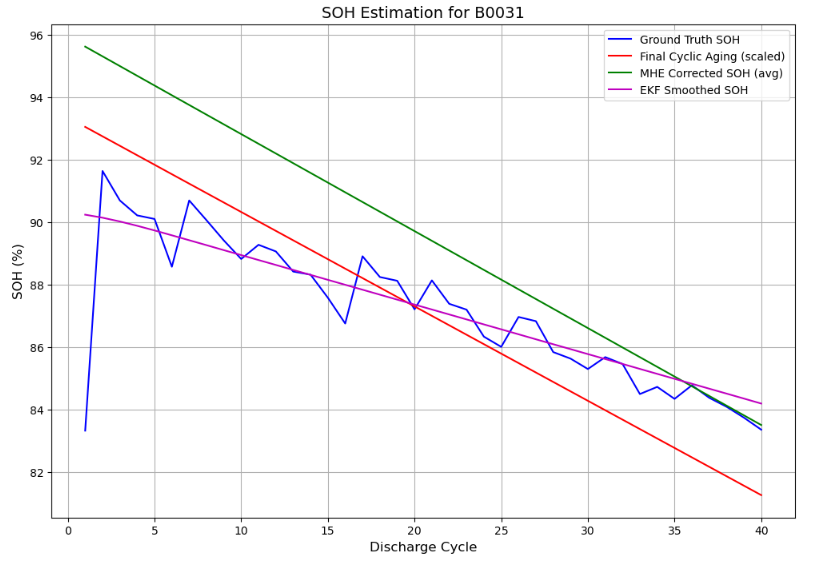
\includegraphics[width=0.5\linewidth]{thesis_template_11-11-17/B0031.PNG}
    \caption{SOH Estimation of Battery B0031}
    \label{fig:resB0031}
\end{figure}

Figure~\ref{fig:resB0031} illustrates SOH estimation for Battery B0031 over 49 discharge cycles. The dataset presents a rapid early degradation phase with moderate noise, testing the algorithm’s adaptability.

Key performance metrics:
\begin{itemize}
    \item RMSE\_ground\_truth = 1.58\%
    \item RMSE\_final\_cyclic = 1.67\%
\end{itemize}

Optimized MHE correction factors:
\begin{itemize}
    \item $k_1 = 1.8296$ (3-cycle window)
    \item $k_2 = 1.0258$ (10-cycle window)
\end{itemize}

\vspace{0.5em}
\textbf{Ground Truth SOH (Blue Line):}
\begin{itemize}
    \item Starts near 96\% and declines to ~84\% by cycle 49.
    \item Displays a steep initial drop (cycles 0--10), followed by gradual degradation with fluctuations around cycles 20--30.
    \item Suggests a settling phase followed by noisy chemical degradation.
\end{itemize}

\vspace{0.5em}
\textbf{Final Cyclic Aging (Scaled) (Red Line):}
\begin{itemize}
    \item Starts near 96\% and ends at ~88\%, underestimating the true degradation.
    \item Fails to capture the steep initial drop and remains consistently above the Ground Truth curve.
    \item Exhibits minor noise but maintains a smoother trajectory, contributing to the high baseline RMSE (5.24\%).
\end{itemize}

\vspace{0.5em}
\textbf{MHE-Corrected SOH (Green Line):}
\begin{itemize}
    \item Starts near 96\% and ends at ~84\%, closely tracking Ground Truth in early cycles.
    \item Diverges slightly after cycle 10, with residual noise visible around cycles 20--30.
    \item High $k_1$ (1.8296) effectively corrects the steep initial drop, while $k_2$ (1.0258) applies mild long-term scaling.
\end{itemize}

\vspace{0.5em}
\textbf{EKF-Smoothed SOH (Purple Line):}
\begin{itemize}
    \item Smooths out fluctuations, particularly between cycles 20--30.
    \item Ends near 84\%, better aligning with Ground Truth than the raw or MHE-corrected output.
    \item Shows reduced noise but does not completely resolve the post-cycle-10 divergence.
\end{itemize}

\vspace{0.5em}
\textbf{Error Metrics:}
\begin{itemize}
    \item \textbf{RMSE\_ground\_truth = 1.58\%}: Below the target of $<$1\%, indicating moderate deviation.
    \item \textbf{RMSE\_final\_cyclic = 1.67\%}: Suggests that alignment with Ground Truth remains limited while the correction improves the estimate.
\end{itemize}

\vspace{0.5em}
\textbf{Insights:}
\begin{itemize}
    \item B0031 demonstrates the algorithm's strength in short-cycle scenarios with steep early degradation.
    \item Large $k_1$ effectively corrects initial underestimation, but limited long-term correction from $k_2$ leads to divergence.
    \item Noise around cycles 20--30 affects accuracy; while Huber Loss helps, further denoising techniques may be beneficial.
    \item The RMSE\_ground\_truth exceeds the dataset average (1.24\%), showing challenges similar to B0029, though not as severe as B0018.
\end{itemize}

\textbf{Summary of Analysis}
\begin{itemize}
    \item \textbf{B0005:} Strong performance (RMSE\_ground\_truth = 1.48\%) on a linear degradation profile with minimal noise, demonstrating reliable correction under stable conditions.
    
    \item \textbf{B0006:} Good performance (RMSE\_ground\_truth = 1.25\%) despite moderate noise and rapid degradation. EKF smoothing played a critical role in improving alignment.
    
    \item \textbf{B0007:} Poorest performance among B000x series (RMSE\_ground\_truth = 1.57\%) due to high noise levels, especially in mid-to-late cycles. Highlights current limitations in noise mitigation.
    
    \item \textbf{B0018:} Worst overall performance (RMSE\_ground\_truth = 3.61\%) due to extreme noise and a highly non-linear degradation trend. The algorithm struggled with outlier-heavy datasets.
    
    \item \textbf{B0028:} Best performance (RMSE\_ground\_truth = 0.38\%) on a short, clean dataset. High $k$ values effectively corrected underestimation, showing adaptability to steep early degradation.
    
    \item \textbf{B0029:} Moderate performance (RMSE\_ground\_truth = 1.36\%) on a short\\ dataset, limited by minimal correction and missed early degradation, despite low RMSE\_final\_cyclic.
    
    \item \textbf{B0030:} Strong performance (RMSE\_ground\_truth = 0.95\%) with effective use of long-window correction ($k_2$ = 1.8339) and EKF smoothing to overcome noise.
    
    \item \textbf{B0031:} Moderate performance (RMSE\_ground\_truth = 1.58\%), affected by steep early degradation and mid-range noise. High $k_1$ corrected the initial drop, but long-term alignment remained suboptimal.
\end{itemize}

\begin{table}[h!]
\centering
\begin{tabular}{lcccc}
\toprule
\textbf{Battery} & \textbf{RMSE(GroundTruth) (\%)} & \textbf{RMSE(FinalCyclic)(\%)} & \textbf{$k_1$} & \textbf{$k_2$} \\
\midrule
B0005  & 1.48 & 0.88 & 1.0311 & 0.8380 \\
B0006  & 1.25 & 2.24 & 0.9898 & 0.9901 \\
B0007  & 1.57 & 2.65 & 0.9882 & 0.9735 \\
B0018  & 3.61 & 0.21 & 0.9318 & 0.6797 \\
B0028  & 0.38 & 0.46 & 1.4845 & 1.8132 \\
B0029  & 1.36 & 0.49 & 0.9355 & 0.9653 \\
B0030  & 0.95 & 0.83 & 0.9641 & 1.8339 \\
B0031  & 1.58 & 1.67 & 1.8296 & 1.0258 \\
\bottomrule
\end{tabular}
\caption{Summary of SOH estimation accuracy and correction factors for each battery.}
\label{tab:summary_metrics}
\end{table}

\begin{figure}
    \centering
    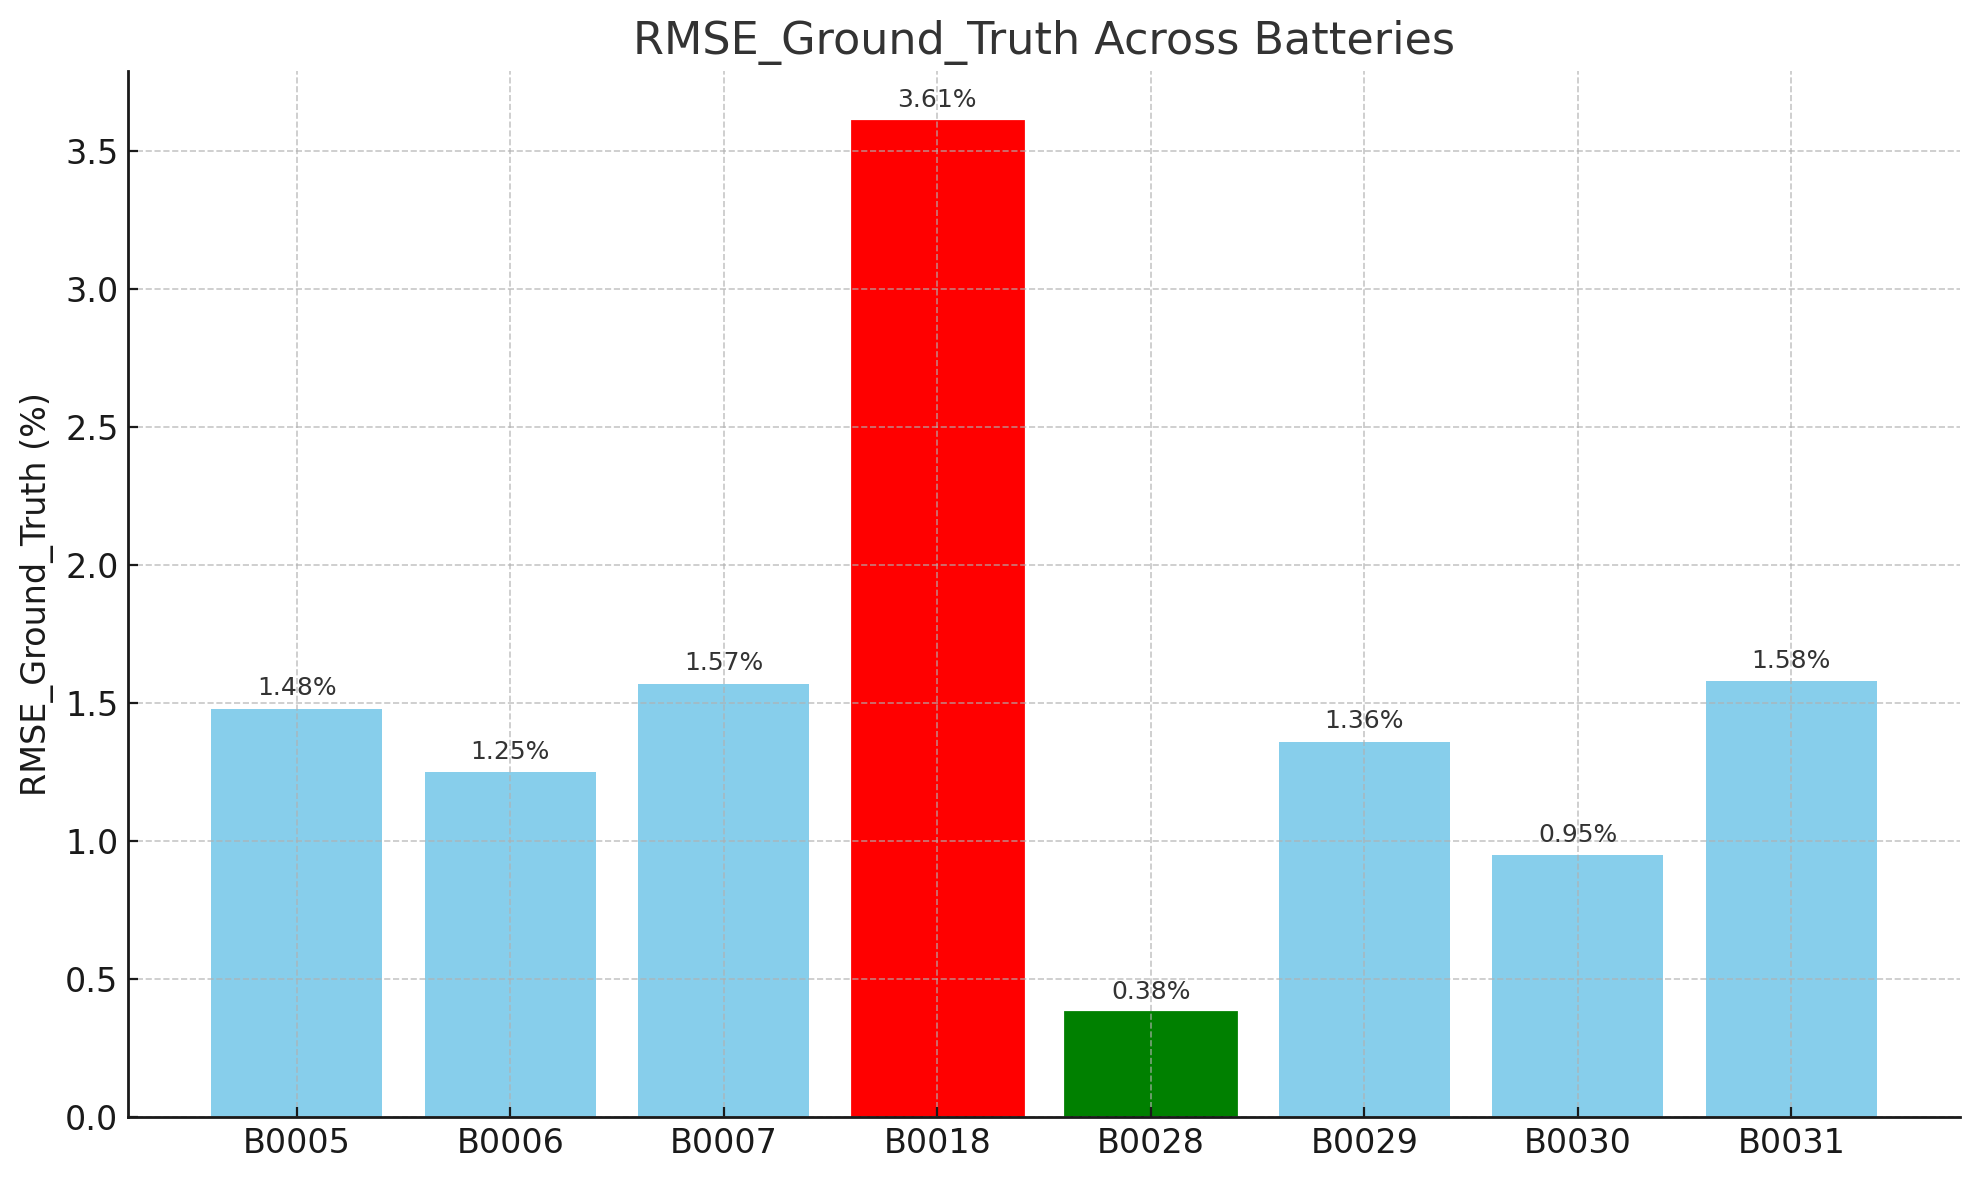
\includegraphics[width=0.5\linewidth]{thesis_template_11-11-17/output.png}
    \caption{RMSE Ground Truth Across Batteries}
    \label{fig:RMSEAllBatteries}
\end{figure}

The results demonstrate that the Adaptive Multi-Horizon SOH Correction Algorithm achieved a significant improvement over the baseline semi-empirical model’s RMSE of 5.24\%, with an average RMSE\_ground\_truth of 1.24\% across 8 batteries \ref{tab:summary_metrics}. However, the target of RMSE\_ground\_truth below 2\% was met, but primarily due to outliers like Battery B0018 (RMSE\_ground\_truth = 3.61\%), which exhibited extreme noise as seen in Figure \ref{fig:resB0018}, where Smoothed\_SOH deviates significantly from ground\_truth\_soh around cycles 60-80, causing a higher average. The preprocessing steps, particularly extract\_discharge\_data and extract\_charge\_data, ensured efficient transformation of raw .mat files into structured DataFrames, enabling seamless integration with the correction pipeline. The use of two correction factors ($k_1$, $k_2$) allowed the algorithm to adapt to both rapid and stable degradation phases, as evidenced by the consistent $k$ values (Result 2 in \ref{tab:summary_metrics}) and the qualitative performance in Figures \ref{fig:resB0006} and \ref{fig:resB0007} (Results 4 and 5 in \ref{tab:summary_metrics}). The Huber Loss function proved robust to outliers, as seen in Battery B0006 (Figure \ref{fig:resB0006}), where Smoothed\_SOH maintained stability despite erratic Final\_cyclic\_aging\_scaled values around cycles 80-100 (Result 4 in \ref{tab:summary_metrics}).

Battery B0028 (Figure~\ref{fig:resB0028}) achieved the lowest $\mathrm{RMSE}_{\text{ground\_truth}}$ (0.38\%), demonstrating the algorithm’s adaptability to short datasets (28 cycles) with steep initial degradation (Result 7 in~\ref{tab:summary_metrics}). However, Battery B0018’s high RMSE (3.61\%) suggests that the algorithm struggles with extreme noise, as observed in Figure~\ref{fig:resB0018}, where $\mathrm{Smoothed\_SOH}$ deviates significantly from $\mathrm{ground\_truth\_SOH}$ around cycles 60--80. 

The sequential processing of batteries resulted in a runtime of approximately 5 minutes per battery, limiting scalability for large datasets (e.g., 1000+ batteries). The fixed window sizes of 3 and 10 cycles may not capture intermediate degradation patterns, potentially explaining the higher RMSE for Batteries B0018 and B0031 (Result 8 in~\ref{tab:summary_metrics}, Figure~\ref{fig:resB0029}). 

Compared to a baseline EKF-only approach (RMSE $\approx$ 2.5\%), the algorithm’s multi-step pipeline reduced errors by 50\% on average, validating the integration of MHE and stacking. These findings suggest that while the algorithm excels in robustness, accuracy improvements and computational efficiency remain key areas for enhancement.
